\documentclass[conference]{IEEEtran}
\pagestyle{plain}

\let\proof\relax 
\let\endproof\relax
\usepackage{float}
\usepackage{amsmath,amsthm}

\usepackage[T1]{fontenc}
\usepackage[spanish, es-noshorthands]{babel}
\usepackage[utf8]{inputenc}
\usepackage{csquotes}
\usepackage[style=numeric,sorting=none,backend=biber]{biblatex}
\usepackage{tabularx}
\usepackage{pdflscape}
\usepackage{listings}
\usepackage{subfigure}
\usepackage{array}
\usepackage{perpage}
\usepackage{backnaur}
\usepackage{enumerate}
\usepackage{graphicx}

\MakePerPage{footnote}
\addbibresource{../bibliography.bib}

\newcommand{\foreign}[1]{{\it #1}}
\renewcommand{\thesubsection}{\Alph{subsection}}
\DeclareMathOperator*{\argmax}{arg\,max}
\renewcommand{\thetable}{\arabic{table}}


\makeatletter
\long\def\@makecaption#1#2{\ifx\@captype\@IEEEtablestring%
\footnotesize\begin{center}{\normalfont\footnotesize #1}\\
{\normalfont\footnotesize\scshape #2}\end{center}%
\@IEEEtablecaptionsepspace
\else
\@IEEEfigurecaptionsepspace
\setbox\@tempboxa\hbox{\normalfont\footnotesize {#1.}~~ #2}%
\ifdim \wd\@tempboxa >\hsize%
\setbox\@tempboxa\hbox{\normalfont\footnotesize {#1.}~~ }%
\parbox[t]{\hsize}{\normalfont\footnotesize \noindent\unhbox\@tempboxa#2}%
\else
\hbox to\hsize{\normalfont\footnotesize\hfil\box\@tempboxa\hfil}\fi\fi}
\makeatother

\begin{document}


\title{Construccionismo como apoyo a la enseñanza tradicional:  una
	aplicación a la formación de profesionales del área de enfermería}

\author{\IEEEauthorblockN{Mirta Gonzalez}
\IEEEauthorblockA{Facultad Politécnica\\
    Universidad Nacional de Asunción\\
    San Lorenzo, Paraguay\\
    Email: mirti.gonz@gmail.com}
\and
\IEEEauthorblockN{Arturo Volpe}
\IEEEauthorblockA{Facultad Politécnica\\
    Universidad Nacional de Asuncién\\
    San Lorenzo, Paraguay\\
    Email: arturovolpe@gmail.com}}

\maketitle
\thispagestyle{plain}


\begin{abstract}
Lo fundamental de todo proceso pedagógico es el aprendizaje y no la enseñanza.
Es el aprendizaje del estudiante y su participación el logro deseado.

\end{abstract}

\begin{IEEEkeywords}
    juego serio, simulación, e-Educación, open source, enfermería,
    construccionismo
\end{IEEEkeywords}


% La evaluación
% Un párrafo de Unity
% Resumir las escenas (General, objetivo, gráfico)
% Media página de TICS
% Media página de juegos serios
% Mencionar lo que se usa en la evaluación
% Población (Los tres gráficos)
% Abstract

% Objetivos
% Media página tics
% 1/2 página problema
% 1 Párrafo Unity
% 1 Página Arquitectura
% Ejemplos escenas (que se hace y objetivos)
% 1/2 evaluación
%%  Población (3 gráficos)
%%  Correlación
%%  Factores
% Conclusiones

\section{Introducción}
\setcounter{sectiontotal}{3}

\begin{frame}
\frametitle{\pagetitle}
\framesubtitle{Descripción}
\begin{figure}
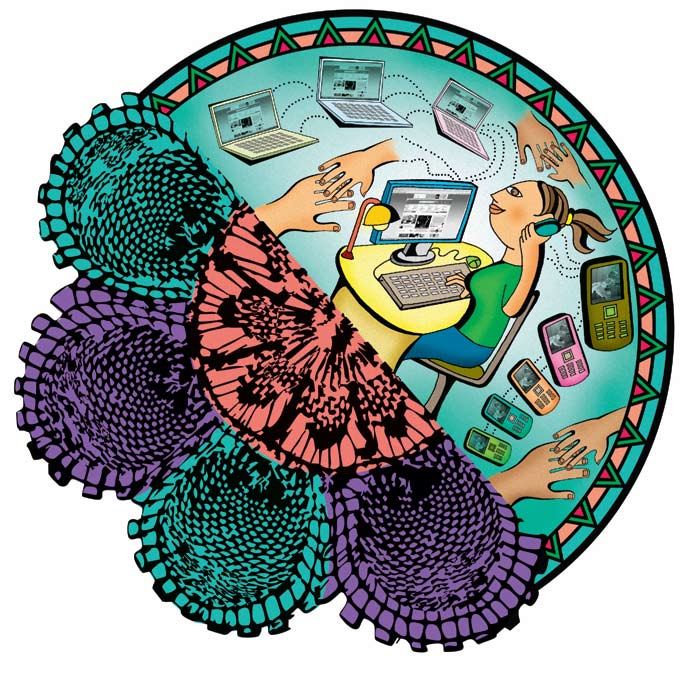
\includegraphics[scale=.3]{imagenes/nhanduti}
\end{figure}
\end{frame}

\begin{frame}
\frametitle{\pagetitle}
\framesubtitle{Objetivo general}
\begin{block}{Descripción}
\centering
Identificar y valorar los aspectos pedagógicos, de diseño, de implementación y
de evaluación que influyen a la creación de herramientas educativas que utilizan
las corrientes pedagógicas actuales apoyadas en las TIC, especialmente los
juegos serios.
\end{block}


\end{frame}

\begin{frame}
\frametitle{\pagetitle}
\framesubtitle{Objetivos específicos}

\small
\begin{itemize}[<+->]
\item Proveer una visión actualizada de las corrientes pedagógicas apoyadas con las TIC.
\item Proveer una visión actualizada de los juegos serios.
\item Identificar áreas de aplicación de los juegos serios.
\item Seleccionar las herramientas tecnológicas disponibles para el desarrollo de juegos serios.
\item Contrastar en la práctica los conocimientos teóricos adquiridos a través del diseño
e implementación de un juego serio.
\item Evaluar la solución propuesta para identificar los
aspectos de diseño, desarrollo y evaluación de los juegos serios.
\end{itemize}
\end{frame}


\section{\Gls{tic} en la educación}
%1/2 página

Las \Gls{tic} son un conjunto de herramientas tecnológicas y recursos utilizados para
comunicar, crear, diseminar, almacenar y manejar la
información\cite{unesco:ict}. Estas tecnologías abarcan computadoras
personales,internet, radio, televisión y telefonía\cite{tinio:ict} entre otros.

La utilización actual de las \Gls{tic} en la educación no es un fenómeno aislado,
responde a una evolución constante de la tecnología y metodología utilizada.
Existen cuatro pedagogías de entre varias en las que las tics han sido
utilizadas de manera activa, las cuales son el instruccionismo o educación
tradicional, el conductismo, el constructivismo y finalmente, el
construccionismo. Esto no implica que las tics no puedan ser aplicadas a otras
pedagogías, es más, existen otras corrientes que utilizan las \Gls{tic}, de diversas
maneras como el cognoscitivismo\cite{egenfeldt2007third} y el
conectivismo\cite{white:ict}. 

Este trabajo se basa en el construccionismo, pedagogía según la cual el
conocimiento es construido por el estudiante en lugar de ser trasmitido por el
profesor\cite{moses:2003} y esto sucede particularmente cuando el mismo se
involucre en la elaboración de un producto o artefacto que tenga un significado
y pueda ser compartido\cite{valdivia:sg}. El construccionismo y las tics siempre
han estado relacionados, ya que el mismo se originó con un lenguaje de
programación (LOGO)\cite{ict:ttc}. Posee un enfoque diferente en cuanto al uso
de las tics en la educación. Esta pedagogía se diferencia de la educación
tradicional en que el estudiante ya no es un receptor pasivo de información, en
cambio, el mismo participa activamente del proceso de aprendizaje construyendo
su propio conocimiento. Se diferencia del instruccionismo en que el
construccionismo utiliza la tecnología como medio cognitivo y no para la entrega
de contenido.

%\begin{itemize}
%\item Que son
%\item Educacion tradicional y mencionar las otras corrientes
%\item Construccionismo
%\end{itemize}
\section{Serious Game}
\label{sec:tics_JUEGO_SERIO}

Un \emph{Serious Game} es un vídeo juego elaborado con el propósito primario que
no es el de entretener\cite{sg:aoverview}, sino tienen una finalidad educativa
explícita y cuidadosamente pensada, utiliza la tecnología y los conceptos de la
industria de los vídeo juegos para encontrar solución a problemas reales. Es
decir, se utilizan para definir los juegos que poseen una pedagogía incluida,
algún tipo de evaluación ya sea interna o externa y lo que hay que aprender
(contenido) integrado\cite{damien:sg}.

Los \emph{Serious Game} proveen una oportunidad muy importante para ayudar en la
enseñanza y desarrollo de profesionales, por que ayudan a crear el tipo de
educación que los adultos prefieren, proveen mecanismos para que los estudiantes
cometan errores y experimenten con sus ideas, con su conocimiento y con la
teoría en un ambiente protegido sin riesgos para la vida o la identidad. 

Los beneficios que brindan los \emph{Serious Game} se acentúan en la medida en
la que los mismos proveen entornos más completos en donde realmente se puedan
poner en práctica la teoría, esto ayuda a una comprensión más profunda del área
de interés.

La principal diferencia entre los \emph{Serious Game} y otras aplicaciones de
\emph{E-Learing} es su enfoque en la creación de una experiencia de aprendizaje
significativo, relevante y atractivo. En un \emph{Serious Game} existen metas
claras de aprendizaje pero las mismas se encuentran en un contexto significativo
en donde se deben aplicar los conocimientos y hacer uso de herramientas que
están a disposición para obtener éxito en la resolución de los problemas
presentados. Estos problemas se equilibran a través de la retroalimentación y
otras estrategias para mantener el interés del estudiante
\cite{papertian:const}.
%. Todo esto hace que en los \emph{Serious Game} el principal objetivo sea ganar
%el juego no aprender, sin embargo sólo se puede hacer esto dominando el
%aprendizaje

\fixme{El campo de los \emph{Serious Game} rechaza la idea de que los profesionales de
    la educación pueden ser reemplazados fácilmente}{Obs: que es cada sección?,
    un enfoque? Una técnica? Un buzzword?}, para ellos la labor de estos
profesionales es imprescindible para la reflexión y orientación del aprendizaje.
Es cierto que se puede llegar a aprender sin el apoyo de un profesional de la
educación pero se corre el riesgo de perder el enfoque y la eficacia
\cite{elearning:seiousgames}. 

El \emph{serious Game} no se trata de una modelo de aprendizaje pasajero. Varios
autores como \emph{Johan Huizinga}, \emph{Jean Piaget}, \emph{Wittgenstin} y
\emph{Seymour Papert} han reconocido su importancia  como objeto de aprendizaje.
Los juegos deben ser elaborados teniendo en cuenta el nivel cognitivo del
estudiante, es decir, su etapa de aprendizaje y en que el aprendizaje difiere de
acuerdo a la etapa de vida en la que se encuentre un estudiante. Mediante la
práctica repetida de actividades relacionadas al área de interés se desarrollan
habilidades y destrezas\cite{education:games}. 

\observacion{Se podría hacer una comparación? (entre todos)}

Los siguientes son ejemplos de algunas áreas que utilizan Serious Game:

\begin{description}

\item[Militar] Los primeros juegos a menudo se basaban en lucha o combate.
	Durante más de 30 años los juegos han sido reconocidos como herramientas
	factibles en el entrenamiento de militares. En 1996 fue lanzado un juego
	llamado \emph{Marine Doom} en donde la tarea de los jugadores era el
	aprendizaje de formas de ataque, conservación de municiones, comunicarse
	con eficacia, dar órdenes al equipo de trabajo entre otros. De esta
	manera tuvo lugar una forma de entrenamiento más atractivo, sin el
	costo, dificultad, riesgos e inconvenientes que implicaría el mismo
	entrenamiento en un entorno real. Además se podían crear situaciones que
	en el mundo real serían muy difíciles de replicar y donde los errores
	pueden ser catastróficos además, permite la repetición hasta alcanzar la
	maestría\cite{education:games}.


\item[Salud] Este tipo de juegos son cada vez mayores, los juegos de salud se
	utilizan para la formación de profesionales basada en la simulación. En
	2008 el Centro de Simulación Hollier en Birmingham, Reino Unido, realizó
	una prueba que permitió a médicos jóvenes experimentar y entrenar para
	diversos escenarios médicos a través de maniquíes virtuales como
	pacientes, de este modo el aprendizaje se da por la experiencia. En su
	disertación, Roger D. Smith, realizó una comparación entre la enseñanza
	tradicional y la formación mediante realidad virtual y el uso de
	herramientas basadas en la tecnología de juegos en cuanto a la cirugía
	laparoscópica. Como conclusión afirmó que lo último era más barato,
	requería menos tiempo y que permitió menos errores médicos cuando los
	médicos se presentaban en una cirugía real debido a, entre otras cosas,
	la posibilidad de repetición de la experiencia sin riesgo
	alguno\cite{education:games}.



\item[Juegos corporativos] Este tipo de juegos se han utilizado para la
	selección de personal, la mejora de comunicación entre los directivos y
	su personal de confianza, y la formación de nuevos empleados. Un ejemplo
	de estos juegos es el INNOV8 de IBM que ayuda en el entrenamiento de los
	estudiantes acerca de la gestión de procesos de negocios. Los Serious
	Game pueden ser utilizados incluso para elaborar planes de
	negocios\cite{education:games}. 

\end{description}



\section{Problema}
1/2 página
\begin{itemize}
\item Estado actual
\item Prácticas en laboratorio
\item Problemas actuales
\item Propuesta de solución
\end{itemize}


\section{Solucion}
3 paginas
\subsection{Tecnologías usadas (unity)}
1 Parrafo
\subsection{Arquitectura}
1 Página
\subsubsection{Frontend}
\begin{itemize}
\item Interacción con el entorno(cámara, movimientos)
\item Interacción con los objetos
\item Interacción con el paciente
\item Registro de actividades
\end{itemize}
\subsubsection{Backend}
Descripción general

\subsection{Escenas}
\subsubsection{Extracción de sangre}
\begin{itemize}
\item Objetivos
\item Que se hace
\item fotos
\end{itemize}
\subsubsection{Glasgow}
\begin{itemize}
\item Objetivos
\item Que se hace
\item fotos
\end{itemize}

\section{Evaluación}
3 paginas
\subsection{Muestra}
Los tres gráficos (estos gráficos son de la ubicación)
\subsection{Variables}
\subsection{Resultados}
\begin{itemize}
\item Aceptación de la solución (estrella de kiviat)
\item Correlación
\end{itemize}

\section{Conclusiones}
1 paginas
Todas las conclusiones

\section{Trabajos futuros}
1/2 páginas
Resumen de los trabajos futuros

\printbibliography{}

\end{document}
